\section{Virtual Private Networks}

\subsection{Introduction to VPNs}

\begin{definition}{Virtual Private Network (VPN)}\\
A VPN is a private network created within a public network infrastructure:
\begin{itemize}
    \item \textbf{Private} - External parties cannot read or modify transmitted data
    \item \textbf{Virtual} - Privacy is achieved through cryptography, not dedicated links
    \item Creates an encrypted tunnel between endpoints
    \item Allows secure access to resources across untrusted networks
\end{itemize}
\end{definition}

\begin{concept}{VPN Use Cases}\\
Common VPN use cases include:
\begin{itemize}
    \item Connecting remote offices or branches to a main corporate network
    \item Allowing partner organizations limited access to internal resources
    \item Enabling remote employees to securely access company resources
    \item Protecting privacy when using public Wi-Fi networks
    \item Bypassing geographical restrictions on content
\end{itemize}
\end{concept}

\begin{theorem}{VPN Core Concepts}\\
Key VPN characteristics include:
\begin{itemize}
    \item VPNs connect networks (or a host to a network), not just individual hosts
    \item VPN endpoints (gateways) establish and maintain the secure tunnel
    \item Internal hosts typically require no special configuration
    \item Traffic is encrypted between VPN endpoints
    \item VPNs often hide internal addressing with NAT
\end{itemize}
\end{theorem}

\subsection{VPN Protocols}

\begin{definition}{VPN Protocol Types}\\
Several protocols are commonly used to implement VPNs:
\begin{itemize}
    \item \textbf{IPsec} - IP Security protocol suite operating at the network layer
    \item \textbf{OpenVPN} - SSL/TLS-based solution running at the application layer
    \item \textbf{WireGuard} - Modern, high-performance VPN protocol
    \item \textbf{Proprietary protocols} - Vendor-specific implementations
\end{itemize}
\end{definition}

\subsection{IPsec VPNs}

\begin{definition}{Internet Protocol Security (IPsec)}\\
IPsec is an IETF standard protocol suite for secure IP communications:
\begin{itemize}
    \item Operates at the network layer (Layer 3)
    \item Provides authentication, integrity, and confidentiality
    \item Includes key exchange mechanism (Internet Key Exchange, IKE)
    \item Supported by most operating systems and network devices
\end{itemize}
\end{definition}

\begin{concept}{IPsec Components}\\
IPsec consists of several components:
\begin{itemize}
    \item \textbf{Authentication Header (AH)} - Provides authentication and integrity (rarely used)
    \item \textbf{Encapsulating Security Payload (ESP)} - Provides encryption, authentication, and integrity
    \item \textbf{Internet Key Exchange (IKE)} - Handles key exchange and security association negotiation
    \item \textbf{Security Associations (SA)} - Parameters for secure communication
\end{itemize}

ESP provides confidentiality, authentication, and integrity protection for IP packets. It operates at the network layer and can protect entire IP packets in tunnel mode or just the payload in transport mode.

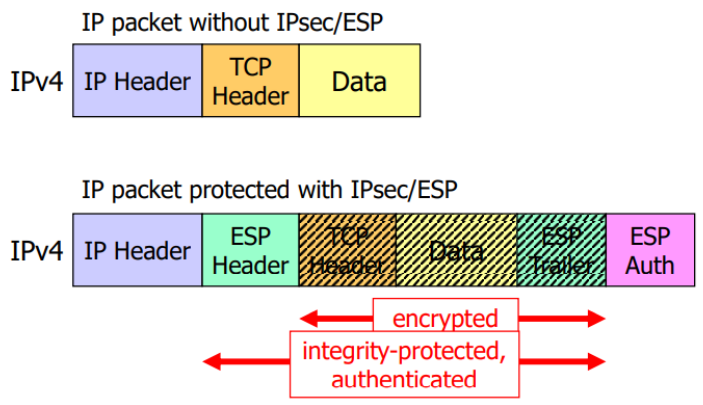
\includegraphics[width=\linewidth]{IPsec.png}

Sequence numbers in IPsec are used to order packets and drop duplicates, providing replay protection:

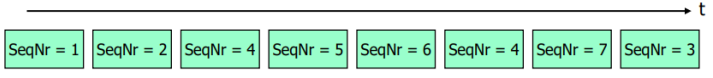
\includegraphics[width=\linewidth]{IPsec_sequence_nr.png}
\end{concept}

\begin{theorem}{IPsec vs. TLS Comparison}\\
IPsec and TLS differ in several key aspects:
\begin{itemize}
    \item \textbf{Layer} - IPsec works at the network layer, TLS at the transport/application layer
    \item \textbf{Protection scope} - IPsec protects all IP traffic between hosts, TLS protects specific application connections
    \item \textbf{Implementation} - IPsec requires kernel integration, TLS runs in user space
    \item \textbf{Configuration} - IPsec typically requires more complex configuration
\end{itemize}
\end{theorem}

\begin{concept}{IPsec Modes}\\
IPsec operates in two primary modes:
\begin{itemize}
    \item \textbf{Transport Mode}:
    \begin{itemize}
        \item Protects the payload of the IP packet
        \item Original IP header remains intact
        \item Typically used for host-to-host communications
    \end{itemize}
    \item \textbf{Tunnel Mode}:
    \begin{itemize}
        \item Protects the entire original IP packet
        \item Encapsulates the original packet in a new IP packet
        \item Typically used for network-to-network (gateway-to-gateway) VPNs
        \item Hides internal IP addressing from eavesdroppers
    \end{itemize}
\end{itemize}
\end{concept}

\begin{code}{IPsec ESP Packet Structure in Tunnel Mode}\\
\begin{lstlisting}[language=C, style=basesmol]
/* Original IP Packet */
struct original_ip_packet {
    struct ip_header original_ip_header;
    struct tcp_header tcp_header;        // Or other protocol
    uint8_t data[VARIABLE_LENGTH];
};

/* IPsec ESP Packet in Tunnel Mode */
struct ipsec_esp_tunnel_packet {
    struct ip_header new_ip_header;      // New header for routing between gateways
    struct esp_header {                  // ESP Header
        uint32_t spi;                    // Security Parameters Index
        uint32_t sequence_number;        // Sequence number for replay protection
    } esp_header;
    
    /* Encrypted portion begins */
    struct original_ip_packet original_packet;  // The entire original packet
    
    uint8_t padding[0-255];              // Padding to block size
    uint8_t pad_length;                  // Number of padding bytes
    uint8_t next_header;                 // Type of the encapsulated header
    /* Encrypted portion ends */
    
    uint8_t integrity_check_value[VARIABLE_LENGTH];  // Authentication data
};
\end{lstlisting}
\end{code}

\begin{KR}{IPsec VPN Setup Process}\\
\paragraph{Phase 1: IKE Security Association}
\begin{itemize}
    \item Exchange cryptographic algorithms and parameters
    \item Authenticate peers (pre-shared keys or certificates)
    \item Establish a secure channel for Phase 2
    \item Generate keying material
\end{itemize}

\paragraph{Phase 2: IPsec Security Association}
\begin{itemize}
    \item Negotiate IPsec security parameters
    \item Establish IPsec SAs for data protection
    \item Define traffic selectors (which traffic to protect)
\end{itemize}

\paragraph{Data Exchange}
\begin{itemize}
    \item Encrypt and authenticate data according to SA parameters
    \item Encapsulate traffic based on tunnel or transport mode
    \item Process incoming encrypted traffic
\end{itemize}

\paragraph{SA Maintenance}
\begin{itemize}
    \item Renew SAs before expiration
    \item Handle dead peer detection
    \item Manage rekeying
\end{itemize}
\end{KR}

\subsection{OpenVPN}

\begin{definition}{OpenVPN}\\
OpenVPN is an open-source VPN solution:
\begin{itemize}
    \item Started as an open-source project in 2002
    \item Uses SSL/TLS for security and key exchange
    \item Operates at the application layer
    \item Creates a virtual network interface in user space
    \item Available for all major operating systems
\end{itemize}
\end{definition}

\begin{concept}{OpenVPN Architecture}\\
OpenVPN's architecture includes several key components:
\begin{itemize}
    \item \textbf{Virtual network interfaces} (TUN/TAP) to capture and inject network traffic
    \item \textbf{SSL/TLS library} for authentication and key exchange
    \item \textbf{Control channel} for management communication
    \item \textbf{Data channel} for encrypted user traffic
    \item \textbf{Configuration system} for defining connection parameters
\end{itemize}
\end{concept}

\begin{theorem}{OpenVPN Protocol Features}\\
OpenVPN offers several protocol features:
\begin{itemize}
    \item Can operate over UDP (default, port 1194) or TCP
    \item Uses SSL/TLS for authentication and key exchange
    \item Implements reliability mechanisms when using UDP
    \item Employs OpenSSL for cryptographic operations
    \item Supports various authentication methods:
    \begin{itemize}
        \item Pre-shared static keys
        \item Certificate-based authentication
        \item Username/password authentication
        \item Multi-factor authentication
    \end{itemize}
\end{itemize}
\end{theorem}

\begin{code}{OpenVPN Packet Format}\\
\begin{lstlisting}[language=C, style=basesmol]
/* OpenVPN Packet Structure */
struct openvpn_packet {
    uint16_t packet_length;       // Length of the entire packet
    uint8_t opcode;               // Operation code (message type + key ID)
    /* 
     * Opcode bits:
     * - First 5 bits: Message type (control, ACK, data)
     * - Last 3 bits: Key ID to identify encryption key set
     */
    
    /* Payload (varies by message type) */
    union {
        /* For control messages (handshake) */
        struct {
            uint8_t session_id[8];      // Session identifier
            uint32_t packet_id;         // Packet identifier for replay protection
            uint8_t hmac[20];           // HMAC for message authentication
            uint8_t tls_payload[];      // TLS handshake data
        } control_message;
        
        /* For data messages */
        struct {
            uint32_t sequence_number;   // Anti-replay sequence number
            uint8_t encrypted_payload[]; // Encrypted IP packet
            uint8_t hmac[];             // HMAC for message authentication
        } data_message;
        
        /* For ACK messages */
        struct {
            uint8_t session_id[8];      // Session identifier
            uint32_t packet_id_array[]; // Array of acknowledged packet IDs
        } ack_message;
    } payload;
};
\end{lstlisting}
\end{code}

\subsection{WireGuard}

\begin{definition}{WireGuard}\\
WireGuard is a modern VPN protocol designed for simplicity and performance:
\begin{itemize}
    \item Developed in 2015 and integrated into Linux kernel in 2020
    \item Uses state-of-the-art cryptography (ChaCha20, Poly1305, Curve25519)
    \item Minimalist design with a small codebase (approximately 4,000 lines)
    \item Provides high performance with lower overhead
    \item Offers better roaming capabilities
\end{itemize}
\end{definition}

\begin{concept}{WireGuard Architecture}\\
WireGuard's architecture focuses on simplicity:
\begin{itemize}
    \item Operates at the network layer (Layer 3)
    \item Implements a "cryptokey routing" concept
    \item Uses public key authentication
    \item Always employs perfect forward secrecy
    \item Maintains a simple, stateless design
\end{itemize}
\end{concept}

\begin{theorem}{WireGuard Features}\\
Key features of WireGuard include:
\begin{itemize}
    \item \textbf{Simplified cryptography} - No cipher negotiation, uses fixed set of modern algorithms
    \item \textbf{Fast handshake} - 1-RTT handshake under normal circumstances
    \item \textbf{Clean, minimal codebase} - Easier to audit and more secure
    \item \textbf{Connection-less design} - No persistent connection state
    \item \textbf{Stealth operation} - No response to unauthenticated packets
    \item \textbf{DoS mitigation} - Cookie challenge mechanism
    \item \textbf{Seamless roaming} - Maintains connections across network changes
\end{itemize}
\end{theorem}

\begin{KR}{Basic WireGuard Configuration}\\
\paragraph{Interface Setup}
\begin{itemize}
    \item Generate public/private key pair
    \item Create WireGuard network interface
    \item Assign IP address to interface
    \item Configure listening port
\end{itemize}

\paragraph{Peer Configuration}
\begin{itemize}
    \item Add peer's public key
    \item Configure allowed IP ranges for cryptokey routing
    \item Set endpoint address if known
    \item Configure optional parameters (keepalive, preshared key)
\end{itemize}

\paragraph{Routing Configuration}
\begin{itemize}
    \item Add routes for traffic to use the WireGuard interface
    \item Configure firewall rules if necessary
    \item Enable packet forwarding if needed
\end{itemize}

\paragraph{Activation}
\begin{itemize}
    \item Bring up the WireGuard interface
    \item Test connectivity
    \item Configure for automatic startup
\end{itemize}
\end{KR}

\begin{examplecode}{Basic WireGuard Configuration}\\
\begin{lstlisting}[language=bash, style=basesmol]
# Generate private and public keys
wg genkey | tee privatekey | wg pubkey > publickey

# Create WireGuard interface
ip link add dev wg0 type wireguard

# Configure interface
ip address add 10.0.0.1/24 dev wg0
wg set wg0 \
    private-key ./privatekey \
    listen-port 51820

# Add peer
wg set wg0 peer PEER_PUBLIC_KEY \
    allowed-ips 10.0.0.2/32 \
    endpoint example.com:51820 \
    persistent-keepalive 25

# Activate interface
ip link set up dev wg0

# Add route (if needed)
ip route add 192.168.0.0/24 via 10.0.0.2

# Save configuration to file
wg showconf wg0 > wg0.conf
\end{lstlisting}
\end{examplecode}

\subsection{Comparing VPN Protocols}

\begin{concept}{Protocol Comparison}\\
IPsec, OpenVPN, and WireGuard have different characteristics:
\begin{itemize}
    \item \textbf{IPsec}:
    \begin{itemize}
        \item Pro: Widely supported, mature standard
        \item Pro: Hardware acceleration in many devices
        \item Con: Complex implementation and configuration
        \item Con: May be blocked by restrictive firewalls
    \end{itemize}
    \item \textbf{OpenVPN}:
    \begin{itemize}
        \item Pro: Cross-platform compatibility
        \item Pro: Runs in user space
        \item Pro: Works well through firewalls (can use TCP port 443)
        \item Con: Slower performance than IPsec and WireGuard
    \end{itemize}
    \item \textbf{WireGuard}:
    \begin{itemize}
        \item Pro: Superior performance and simplicity
        \item Pro: Modern cryptography by default
        \item Pro: Small, auditable codebase
        \item Con: Less mature than alternatives
        \item Con: Fixed cryptographic algorithms
    \end{itemize}
\end{itemize}
\end{concept}

\subsection{VPN Deployment Scenarios}

\begin{concept}{Site-to-Site VPN}\\
Site-to-site VPNs connect entire networks:
\begin{itemize}
    \item Connect branch offices to headquarters
    \item Connect partner organizations' networks
    \item Implemented using VPN gateways at each location
    \item Transparent to end users
    \item Typically always-on connections
\end{itemize}
\end{concept}

\begin{concept}{Remote Access VPN}\\
Remote access VPNs connect individual users to a network:
\begin{itemize}
    \item Enable employees to work remotely
    \item Allow access to internal resources from outside
    \item Implemented using VPN client software on user devices
    \item Often use dynamic IP addressing with virtual addresses
    \item Typically on-demand connections
\end{itemize}
\end{concept}

\begin{example}
A multinational company uses a hybrid VPN setup to secure its communications. For connecting its headquarters to branch offices in different countries, it deploys site-to-site IPsec VPNs with AES-256 encryption and certificate-based authentication. These connections are always active and transparent to users.

For its remote employees, the company provides OpenVPN access using two-factor authentication. When traveling employees connect from hotel Wi-Fi networks, the OpenVPN client encrypts all their traffic and tunnels it to the corporate network. The system assigns each connected user a virtual IP address (10.3.0.x) from a dedicated pool, enabling internal systems to apply appropriate access controls based on these addresses.
\end{example}

% Duplicate content removed - comprehensive VPN coverage is provided above